\section*{Anexo}
\appendix
\section{Líneas de trabajo descartadas}
\subsection{Caracterización morfológica de las shells con HST}
\label{sec:anexo}
Como se ha descrito en el texto, el procedimiento para medir las propiedades de la shell principal consistió en delimitar el contorno que describe en la imagen residual del filtro F277W de JWST y medir el flujo sobre la imagen original en todos los filtros. Sin embargo, este no era el tratamiento que pretendíamos hacer a priori. El análisis original consistía en obtener una imagen residual en todos los filtros de fotometría y medir el flujo sobre dicha imagen residual, en lugar de sobre las imágenes originales. Dicho procedimiento obtuvo resultados satisfactorios en los filtros de JWST. Sin embargo, al aplicar el mismo análisis para el filtro F160W de HST/WFC3, GALFIT modela una galaxia más alargada (\(b/a = 0,38\)) que hace desaparecer la shell secundaria y afecta gravemente al centro de la principal. Además, no es capaz de eliminar satisfactoriamente la luz de la BCG al norte y al sur, por lo que tampoco es posible distinguir esta shell de la BCG. Este ajuste es estable bajo grandes variaciones de los parámetros iniciales y la aplicación de máscaras (zonas no tenidas en cuenta en el ajuste) en determinadas regiones. Presentamos el resultado en la Figura \ref{hst160}.\par 


\begin{figure}[h]
\centering
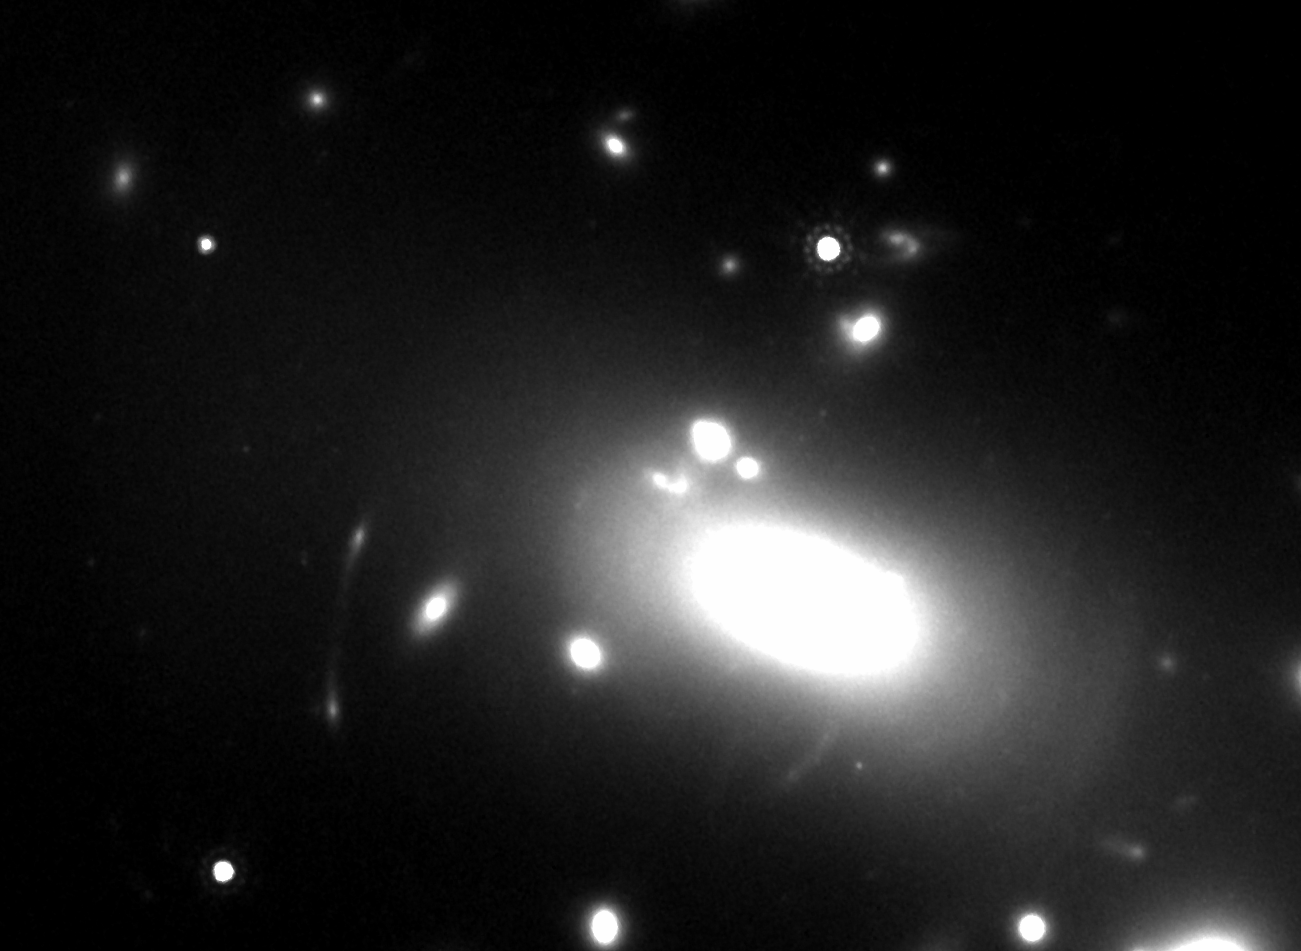
\includegraphics[trim={300 0 0 200}, clip, width=0.45\textwidth]{hst160.png}
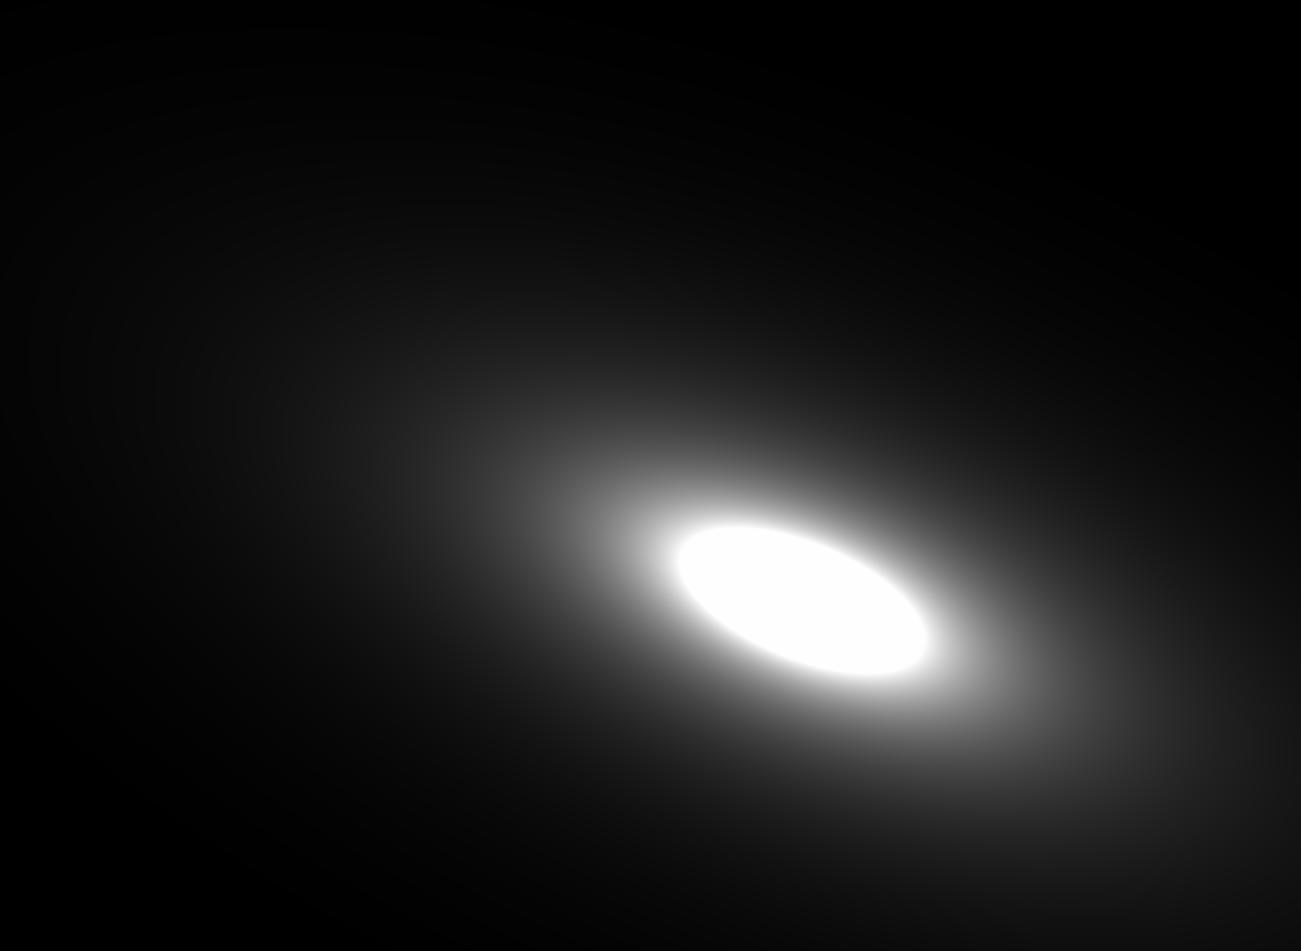
\includegraphics[trim={300 0 0 200}, clip, width=0.45\textwidth]{hst160_elipse.png} \\
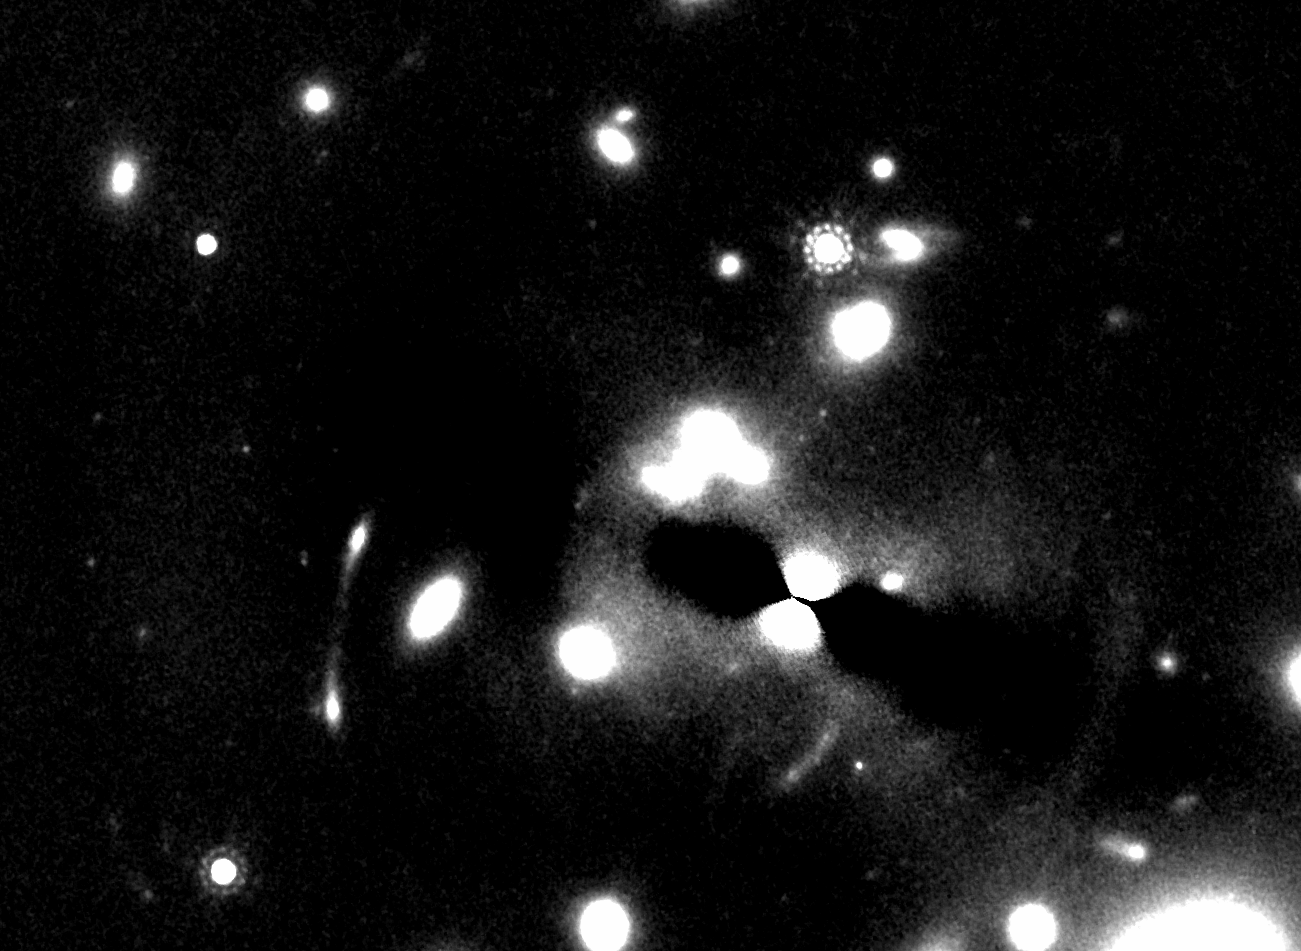
\includegraphics[trim={300 0 0 200}, clip, width=0.5\textwidth]{hst160_sinbcg.png}
\caption{Fila superior, izquierda: imagen de la BCG de \clust{} en el filtro F160W de HST con una escala de 0-0,15 e\(^{-}\)/s. Fila superior, derecha: modelo de GALFIT de la BCG de \clust{}, con la misma escala. En este caso, el modelo es más alargado que la BCG de la imagen original. Inferior: imagen residual resultante de restar la segunda imagen a la primera, con una escala de 0-0,03 e\(^{-}\)/s. El modelo la BCG es claramente inadecuado y no permite distinguir con claridad las estructuras. \label{hst160}}
\end{figure}
\noindent

Estas dificultades se repiten en el resto de filtros de HST, por lo que, como se menciona en el texto, suponen una demostración palpable de la potencia del telescopio James Webb como herramienta para la caracterización de objetos de bajo brillo superficial. Obviamente, con estas circunstancias el planteamiento original quedó descartado, lo que no impidió obtener resultados significativos. \par

\subsection{Métodos alternativos para la eliminación de las contribuciones espurias al flujo de la shell} \label{sec:chefs}
Otra cuestión relevante en el análisis de la shell, especialmente si se cumplieran las condiciones del anterior apartado, es la eliminación de las galaxias presentes en la shell principal. Como describimos en el texto, en nuestro análisis optamos por enmascararlas. Sin embargo, también existe la posibilidad de modelar su perfil lumínico para, en la medida de lo posible, aislarlo y eliminarlo, y de ese modo reducir el área enmascarada. La forma más directa es hacerlo con GALFIT, aplicando el mismo procedimiento que utilizamos con la BCG sobre la imagen residual de esta. En este caso tenemos en cuenta seis modelos de galaxias al mismo tiempo (es necesario combinar las cuatro galaxias de la zona central en dos modelos), que mostramos, junto con su imagen residual, en la Figura \ref{fig:galgalfit}. Vemos un buen acuerdo entre el modelo y la imagen original de F277W (Figura \ref{jwst277}, inferior), y en la imagen residual reducimos notablemente el área que podría dar problemas. \par


\begin{figure}[h!]
\centering
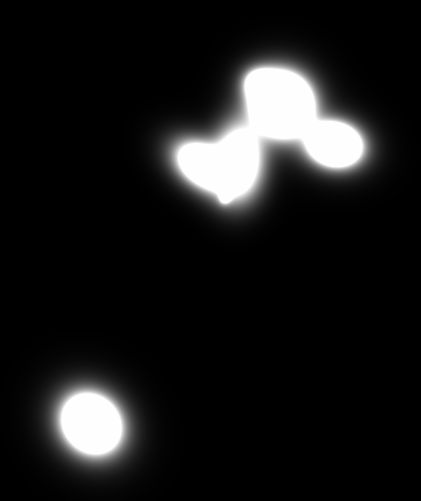
\includegraphics[trim={0 0 0 0}, clip, width=0.45\textwidth]{galaxiasgalfit_modelo.png}
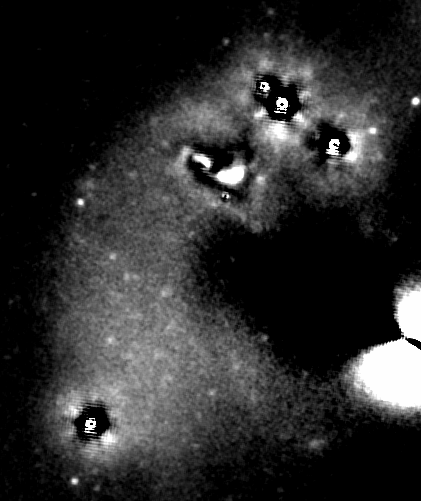
\includegraphics[trim={0 0 0 0}, clip, width=0.45\textwidth]{galaxiasgalfit.png}
\caption{Modelos de GALFIT para las galaxias superpuestas sobre la shell principal (izquierda) y su imagen residual para F277W (derecha), ambas con una escala de 0-0,2 MJy/sr. Se tienen en cuenta seis modelos distintos que son capaces de reducir notablemente la contribución de las galaxias que se observaba en la Figura \ref{jwst277}. \label{fig:galgalfit}}
\end{figure}
\noindent

Sin embargo, al ser imposible conseguir una reducción de la BCG con la misma calidad en las imágenes de HST, no es posible llevar a cabo este análisis, ya que las galaxias no quedan bien modeladas. En cualquier caso, tampoco era viable aplicar el procedimiento para el cubo de datos de MUSE. Otra alternativa, más automatizada, que se exploró fue utilizar un algoritmo basado en objetos matemáticos conocidos como CHEFs \citep{jimenez-tejaNewToolImage2012}, utilizado en \citet{jimenez-tejaFirstJointMUSE2024} para estimar la forma de la ICL del cúmulo. En la Figura \ref{fig:galchefs} vemos el resultado de aplicar dicho algoritmo a la imagen residual de F277W. Si bien es cierto que el perfil de las galaxias queda más suavizado, el algoritmo extiende la forma de la shell y no está claro que pueda producir un buen análisis. Por ello, dado que finalmente decidimos trabajar con los flujos de las imágenes originales y no es tan necesario maximizar el área de la shell para reducir los errores, optamos por no seguir por esta vía.

\begin{figure}[h!]
\centering
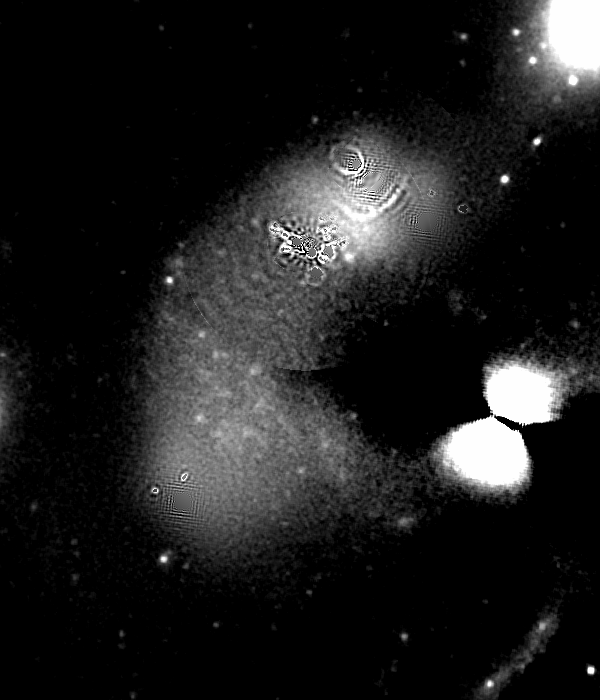
\includegraphics[trim={0 0 0 0}, clip, width=0.45\textwidth]{galaxiaschefs.png}
\caption{Imagen residual resultante de aplicar un algoritmo basado en CHEFs para la eliminación de las galaxias superpuestas sobre la shell principal, con una escala de 0-0,2 MJy/sr. El algoritmo suaviza notablemente todos los bordes del contorno, incluyendo una extensión de la shell en el interior de la parte central. Por este motivo descartamos utilizarlo para medir el flujo sobre la shell. \label{fig:galchefs}}
\end{figure}
\noindent

\section{Mapa de color de la BCG sin filtro gaussiano} \label{sec:colorsingauss}

\begin{figure}[h]
\centering
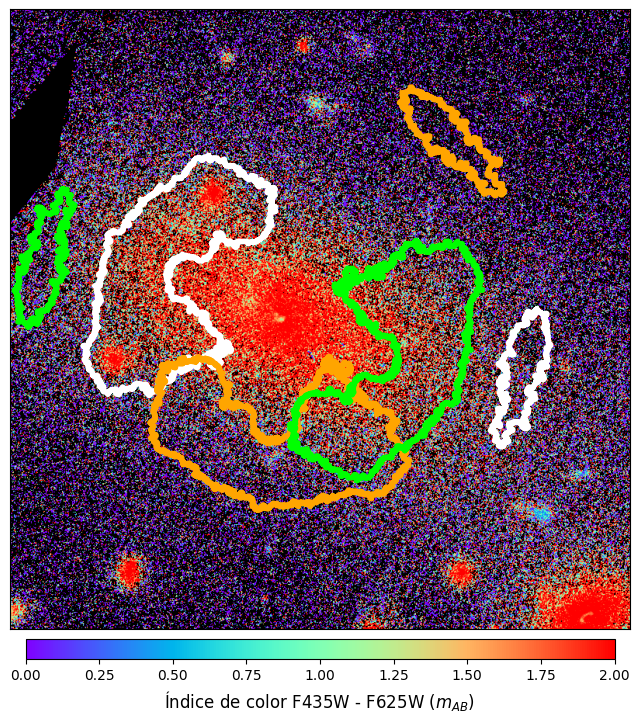
\includegraphics[trim={5 0 5 5}, clip, width=0.7\textwidth]{colorsingauss.png}
\caption{Mapa de color idéntico a la Figura \ref{color}, pero sin haber aplicado el filtro gaussiano de \textit{scipy}. En este caso, los puntos negros se corresponden con píxeles sin un índice de color definido, debido a que en al menos uno de los dos filtros el flujo en ellos es nulo o negativo.\label{colorsingauss}}
\end{figure}
\noindent